% !TEX root = ../main.tex

\section{Introduction}
\label{sec:introduction}
 
In this lab we will venture into the memory of the GPU. Despite the fact that Numbu already uses some basic memory management in the background we will still experiment with it manually. By doing this we should see some improvements in execution times. We will first implement a kernel function that filters a certain signal with and without the use of memory pre-allocation. After that a function previously used will be implemented that can use the pre-existing data on the GPU.

The code repository can be found at: \\
\url{https://github.com/imstevenxyz/geavanceerde-computerarch}

\newpage

\section{Kolmogorov–Zurbenko filter}
\label{sec:Kolmogorov–Zurbenko filter}

The first part of this lab consists of a Kolmogorov–Zurbenko filter that is implemented parallel in a kernel function as seen in code fragment \ref{lst:filterkernel}. This function takes three important arguments, the original signal samples array, the filter coefficients and the result array. The variables that will hold the corresponding data will be transferred to the GPU memory, first alone and then all three together. This will be done using the \code{cuda.to\_device()} method.

\begin{lstlisting}[language=Python,caption={KZ-filter kernel function},label={lst:filterkernel}]
@cuda.jit
def kernel_filter_outputFocus(samples, coeffs, result):
    # Calculate the thread's absolute position within the grid
    x = cuda.threadIdx.x + cuda.blockIdx.x * cuda.blockDim.x

    # Set stride equal to the number of threads we have available in either direction
    stride_x = cuda.gridDim.x * cuda.blockDim.x

    for i in range(x, result.shape[0], stride_x):
        for j in range(coeffs.shape[0]):
            result[i]+=samples[i+j]*coeffs[j]
\end{lstlisting}

The kernel execution timing results are:
\begin{itemize}
    \item No memory management => 0.0027556300163269045
    \item Only the original signal samples transferred => 0.0024497437477111815
    \item Only the coefficients transferred => 0.002444329261779785
    \item Only the result transferred => 0.002314467430114746
    \item Everything transferred => 0.0017078185081481933
\end{itemize}

Of course the transfer of read-only data to the GPU memory also takes time:
\begin{itemize}
    \item Transferring the original signal => 0.00028020620346069336
    \item Total execution time with transfer => 0.002650794982910156
\end{itemize}

By comparing these result we see that the execution time somewhat decreases when all data is transferred. But we should take into account that the transfer itself is not included in the result. When we add the transfer and execution time together we see that it is only faster by a small fraction. 0.00275 compared to 0.00265.

\newpage

In the following figure (\ref{figure:exec_times}) we see the difference in execution times with and without memory management. Transfer time is added to the execution time. Overall, there is a constant improvement in execution time that does not increase of decrease based on the sample set size, at least not one that is directly visible in the graph.

\begin{figure}[H]
    \centering
    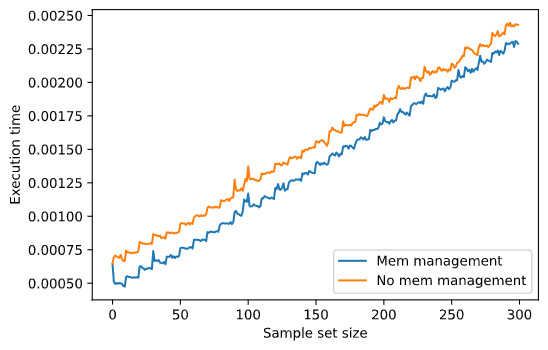
\includegraphics[width=0.7\textwidth]{images/exectimesfilter.png}
    \caption{Execution times}
    \label{figure:exec_times}
\end{figure}
  

\section{DFT}
\label{sec:DFT}

Now two kernel functions are implemented that are executed in sequence after each other that process the same memory transferred with \code{cude.to\_device()}. By doing this the data does not have to be transferred back to the CPU, this gives us of course less overhead. This is useful since both kernel function work hand in hand to calculate one end result and the data should not be transferred unnecessarily.

The timing results of the execution are:
\begin{itemize}
    \item No memory management => 0.11401880025863648
    \item Memory management => 0.11228885889053344
\end{itemize}

There is a small decrease in execution time, but as seen in the previous section we have to take into account the transfer time of the data.

\newpage
\section{Conclusion}
\label{sec:conclusion}

Overall we see that memory management has some improvements and ease of uses. The execution times mostly improve because the transfer is no longer timed directly. Furthermore, Numba itself already does a lot of memory management in the background, maybe not that efficiently. If needed, manual memory management can be used and can in theory greatly improve the execution times when possible and unnecessary data transfers will bottleneck the bus system. Since we use only a small set of samples, the data to transfer is not that big and does of course not create that much overhead. When memory management is used for a lot of data we should see good improvements in the timing results.